\documentclass{article}\usepackage[]{graphicx}\usepackage[]{color}
%% maxwidth is the original width if it is less than linewidth
%% otherwise use linewidth (to make sure the graphics do not exceed the margin)
\makeatletter
\def\maxwidth{ %
  \ifdim\Gin@nat@width>\linewidth
    \linewidth
  \else
    \Gin@nat@width
  \fi
}
\makeatother

\definecolor{fgcolor}{rgb}{0.345, 0.345, 0.345}
\newcommand{\hlnum}[1]{\textcolor[rgb]{0.686,0.059,0.569}{#1}}%
\newcommand{\hlstr}[1]{\textcolor[rgb]{0.192,0.494,0.8}{#1}}%
\newcommand{\hlcom}[1]{\textcolor[rgb]{0.678,0.584,0.686}{\textit{#1}}}%
\newcommand{\hlopt}[1]{\textcolor[rgb]{0,0,0}{#1}}%
\newcommand{\hlstd}[1]{\textcolor[rgb]{0.345,0.345,0.345}{#1}}%
\newcommand{\hlkwa}[1]{\textcolor[rgb]{0.161,0.373,0.58}{\textbf{#1}}}%
\newcommand{\hlkwb}[1]{\textcolor[rgb]{0.69,0.353,0.396}{#1}}%
\newcommand{\hlkwc}[1]{\textcolor[rgb]{0.333,0.667,0.333}{#1}}%
\newcommand{\hlkwd}[1]{\textcolor[rgb]{0.737,0.353,0.396}{\textbf{#1}}}%

\usepackage{framed}
\makeatletter
\newenvironment{kframe}{%
 \def\at@end@of@kframe{}%
 \ifinner\ifhmode%
  \def\at@end@of@kframe{\end{minipage}}%
  \begin{minipage}{\columnwidth}%
 \fi\fi%
 \def\FrameCommand##1{\hskip\@totalleftmargin \hskip-\fboxsep
 \colorbox{shadecolor}{##1}\hskip-\fboxsep
     % There is no \\@totalrightmargin, so:
     \hskip-\linewidth \hskip-\@totalleftmargin \hskip\columnwidth}%
 \MakeFramed {\advance\hsize-\width
   \@totalleftmargin\z@ \linewidth\hsize
   \@setminipage}}%
 {\par\unskip\endMakeFramed%
 \at@end@of@kframe}
\makeatother

\definecolor{shadecolor}{rgb}{.97, .97, .97}
\definecolor{messagecolor}{rgb}{0, 0, 0}
\definecolor{warningcolor}{rgb}{1, 0, 1}
\definecolor{errorcolor}{rgb}{1, 0, 0}
\newenvironment{knitrout}{}{} % an empty environment to be redefined in TeX

\usepackage{alltt}
\usepackage[utf8]{inputenc}
\usepackage[margin=1in]{geometry}
\usepackage{hyperref}
\usepackage{xcolor}
\usepackage{listings}
\usepackage{graphicx}
\usepackage{amsmath}
\pagenumbering{arabic}		
\usepackage{amssymb}
\usepackage{pdfpages}
\usepackage{mathtools}
\usepackage[utf8]{inputenc}
\usepackage{fancyhdr}
\usepackage{lastpage}
 
\pagestyle{fancy}
\fancyhf{}


\lstset{basicstyle=\ttfamily,
  showstringspaces=false,
  commentstyle=\color{red},
  keywordstyle=\color{blue}
}

\title{Problem Set 8}
\author{Alexander Brandt\\SID: 24092167}
\date{December 7 2015}
\IfFileExists{upquote.sty}{\usepackage{upquote}}{}
\begin{document}

\maketitle

Friendly Collaborators: Milos Atz, Alex Ojala and Guillame Baquiast.

\section{}

\subsection{}

We generate several data sets given a linear model, with a random variable signifying noise.   We will input the \(x_i\) and \(y_i\) into both of the models we wish to test.  For each model, we will compute the prediction error and the coverage as follows:
\\\\
Prediction error is the absolute difference between the data and the predicted value, and the coverage can be generated in a non-parametric fashion by selecting, with replacement, n values (n should not be too small) and use order statistics to generate the prediction interval of a given percentage (this is the boostrap).
\\\\
To compare these methods to see which is ``better'' we can generate a mean and variance of both preidiction error and coverage.  We will choose the method which minimizes the variance.
\subsection{}

We choose some linear function \(f\) that we wish to recapitulate with our analysis.  The x-values are generated uniformly on a given range, and the y-values are determined to be \(y_i = f(x_i) + \epsilon_i\).  \(\epsilon_i\) has some large probability of being a ``minor'' error, or a small probability of begin a ``major'' error, giving rise to an outlier value.  We simulate a random variable on the interval 0 to 1, and if it is below some small value (.05, .01, etc.), we greatly increase the value of the magnitude of the error (so if normally \(\epsilon_i\) is \(~\) N(0,1), now it will be something like \(~\) N(0,10).

\section{}

\subsection{}

The pareto decays more slowly than the exponential.  Note: pareto here is graphed in black.

\begin{knitrout}
\definecolor{shadecolor}{rgb}{0.969, 0.969, 0.969}\color{fgcolor}\begin{kframe}
\begin{alltt}
\hlstd{pareto} \hlkwb{<-} \hlkwa{function}\hlstd{(}\hlkwc{x}\hlstd{,} \hlkwc{alpha}\hlstd{,} \hlkwc{beta}\hlstd{) \{}
  \hlkwd{return}\hlstd{(beta} \hlopt{*} \hlstd{(alpha}\hlopt{^}\hlstd{beta)} \hlopt{/} \hlstd{(x}\hlopt{^}\hlstd{(beta}\hlopt{+}\hlnum{1}\hlstd{)))}
\hlstd{\}}

\hlstd{expd} \hlkwb{<-} \hlkwa{function}\hlstd{(}\hlkwc{x}\hlstd{,} \hlkwc{lambda}\hlstd{,} \hlkwc{xshift}\hlstd{) \{}
  \hlkwd{return}\hlstd{( lambda} \hlopt{*} \hlkwd{exp}\hlstd{(} \hlopt{-}\hlstd{lambda} \hlopt{*} \hlstd{(x} \hlopt{-} \hlstd{xshift) ))}
\hlstd{\}}

\hlstd{alpha} \hlkwb{<-} \hlnum{2}
\hlstd{beta} \hlkwb{<-} \hlnum{3}

\hlstd{x} \hlkwb{<-} \hlkwd{seq}\hlstd{(}\hlkwc{from}\hlstd{=}\hlnum{.2}\hlstd{,} \hlkwc{to}\hlstd{=}\hlnum{.5}\hlstd{,} \hlkwc{by}\hlstd{=}\hlnum{.001}\hlstd{)}
\hlkwd{plot}\hlstd{(x,} \hlkwd{pareto}\hlstd{(x,} \hlnum{.5}\hlstd{,} \hlnum{.6}\hlstd{),} \hlkwc{type}\hlstd{=}\hlstr{'l'}\hlstd{,}\hlkwc{ylim}\hlstd{=}\hlkwd{c}\hlstd{(}\hlnum{0}\hlstd{,}\hlnum{6}\hlstd{))}
\hlkwd{lines}\hlstd{(x,} \hlkwd{expd}\hlstd{(x,} \hlnum{10}\hlstd{,} \hlnum{0}\hlstd{),} \hlkwc{col}\hlstd{=}\hlnum{26}\hlstd{)}
\end{alltt}
\end{kframe}
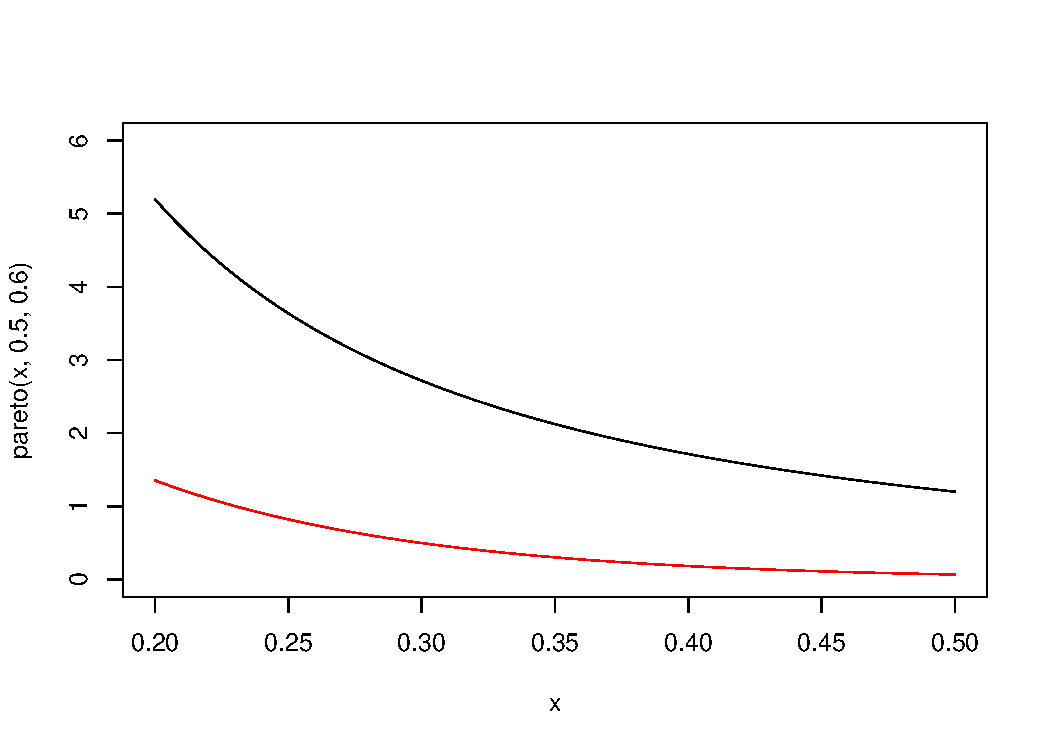
\includegraphics[width=\maxwidth]{figure/unnamed-chunk-1-1} 

\end{knitrout}

\subsection{}

\begin{knitrout}
\definecolor{shadecolor}{rgb}{0.969, 0.969, 0.969}\color{fgcolor}\begin{kframe}
\begin{alltt}
\hlcom{# Rewriting our functions just a bit to take into account the problem}
\hlcom{# statement:}

\hlstd{pareto} \hlkwb{<-} \hlkwa{function}\hlstd{(}\hlkwc{x}\hlstd{,} \hlkwc{alpha}\hlstd{,} \hlkwc{beta}\hlstd{) \{}
  \hlkwd{return}\hlstd{(beta} \hlopt{*} \hlstd{(alpha}\hlopt{^}\hlstd{beta)} \hlopt{/} \hlstd{(x}\hlopt{^}\hlstd{(beta}\hlopt{+}\hlnum{1}\hlstd{)))}
\hlstd{\}}

\hlstd{inverse_cdf_pareto} \hlkwb{<-} \hlkwa{function}\hlstd{(}\hlkwc{p}\hlstd{,} \hlkwc{alpha}\hlstd{,} \hlkwc{beta}\hlstd{) \{}
  \hlkwd{return}\hlstd{( alpha} \hlopt{*} \hlstd{((}\hlnum{1} \hlopt{-} \hlstd{p)} \hlopt{^} \hlstd{(}\hlopt{-}\hlnum{1} \hlopt{/} \hlstd{beta)) )}
\hlstd{\}}

\hlstd{expd} \hlkwb{<-} \hlkwa{function}\hlstd{(}\hlkwc{x}\hlstd{,} \hlkwc{lambda}\hlstd{,} \hlkwc{xshift}\hlstd{) \{}
  \hlkwd{return}\hlstd{( (x} \hlopt{>=} \hlnum{2}\hlstd{)} \hlopt{*} \hlstd{lambda} \hlopt{*} \hlkwd{exp}\hlstd{(} \hlopt{-}\hlstd{lambda} \hlopt{*} \hlstd{(x} \hlopt{-} \hlstd{xshift) ))}
\hlstd{\}}

\hlcom{# This is JUST the inverse cdf for the specific function asked}
\hlstd{inverse_cdf_myexp} \hlkwb{<-} \hlkwa{function}\hlstd{(}\hlkwc{p}\hlstd{) \{}
  \hlkwd{return}\hlstd{(}\hlnum{2} \hlopt{-} \hlkwd{log}\hlstd{(}\hlnum{1}\hlopt{-}\hlstd{p))}
\hlstd{\}}

\hlstd{alpha} \hlkwb{<-} \hlnum{2}
\hlstd{beta} \hlkwb{<-} \hlnum{3}

\hlstd{m} \hlkwb{<-} \hlnum{10000}
\hlstd{us} \hlkwb{<-} \hlkwd{runif}\hlstd{(}\hlkwc{n}\hlstd{=m)}

\hlcom{# Sample our values}
\hlstd{vals} \hlkwb{<-} \hlkwd{inverse_cdf_pareto}\hlstd{(us,} \hlkwc{alpha}\hlstd{=}\hlnum{2}\hlstd{,} \hlkwc{beta}\hlstd{=}\hlnum{3}\hlstd{)}

\hlcom{# Define our functions f and g}
\hlstd{f} \hlkwb{<-} \hlkwd{expd}\hlstd{(vals,} \hlkwc{lambda} \hlstd{=} \hlnum{1}\hlstd{,} \hlkwc{xshift}\hlstd{=}\hlnum{2}\hlstd{)}
\hlstd{g} \hlkwb{<-} \hlkwd{pareto}\hlstd{(vals,} \hlkwc{alpha}\hlstd{=alpha,} \hlkwc{beta}\hlstd{=beta)}

\hlcom{# Contruct our weights, and expectations of X and X^2}
\hlstd{my_weights} \hlkwb{<-} \hlstd{f} \hlopt{/} \hlstd{g}
\hlstd{ex_vals} \hlkwb{<-} \hlstd{vals} \hlopt{*} \hlstd{my_weights}
\hlstd{ex_2_vals} \hlkwb{<-} \hlstd{vals}\hlopt{^}\hlnum{2} \hlopt{*} \hlstd{my_weights}
\hlstd{EX} \hlkwb{<-} \hlkwd{mean}\hlstd{(ex_vals)}
\hlstd{EX2} \hlkwb{<-} \hlkwd{mean}\hlstd{(ex_2_vals)}

\hlkwd{attach}\hlstd{(mtcars)}
\hlkwd{par}\hlstd{(}\hlkwc{mfrow}\hlstd{=}\hlkwd{c}\hlstd{(}\hlnum{1}\hlstd{,}\hlnum{3}\hlstd{))}

\hlcom{# Plot the histograms}
\hlkwd{hist}\hlstd{(ex_vals)}
\hlkwd{hist}\hlstd{(ex_2_vals)}
\hlkwd{hist}\hlstd{(my_weights)}
\end{alltt}
\end{kframe}
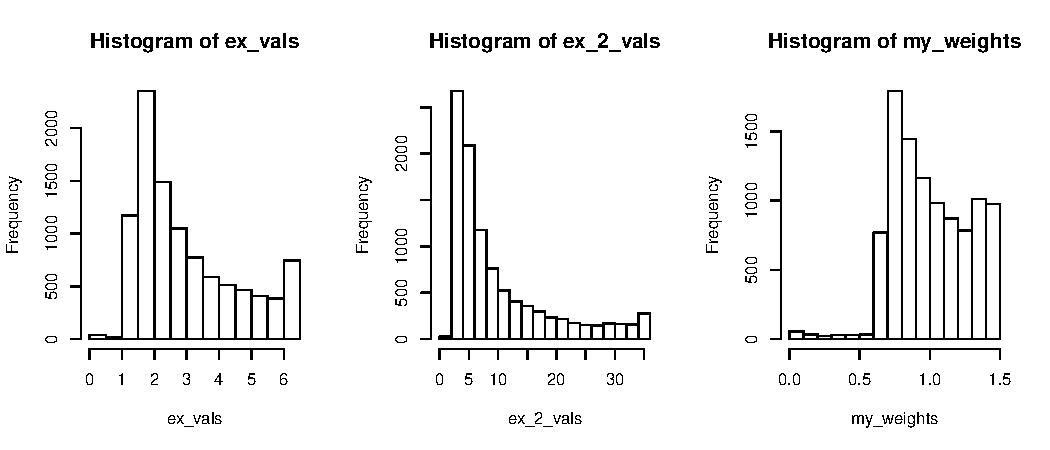
\includegraphics[width=\maxwidth]{figure/unnamed-chunk-2-1} 
\begin{kframe}\begin{alltt}
\hlcom{# Display the values}
\hlstd{EX}
\end{alltt}
\begin{verbatim}
## [1] 3.014705
\end{verbatim}
\begin{alltt}
\hlstd{EX2}
\end{alltt}
\begin{verbatim}
## [1] 10.07258
\end{verbatim}
\end{kframe}
\end{knitrout}

Because we are attempting to perform an importance sampling, we can see our higher weights are sampled more frequently than would be expected from an agnostic sampling of the distribution (in the first scenario).

\subsection{}

\begin{knitrout}
\definecolor{shadecolor}{rgb}{0.969, 0.969, 0.969}\color{fgcolor}\begin{kframe}
\begin{alltt}
\hlcom{# c)}
\hlcom{# Almost exactly the same as above, now we just switch our}
\hlcom{# definitions of g and f:}

\hlstd{m} \hlkwb{<-} \hlnum{10000}
\hlstd{us} \hlkwb{<-} \hlkwd{runif}\hlstd{(}\hlkwc{n}\hlstd{=m)}

\hlstd{vals} \hlkwb{<-} \hlkwd{inverse_cdf_myexp}\hlstd{(us)}

\hlstd{g} \hlkwb{<-} \hlkwd{expd}\hlstd{(vals,} \hlkwc{lambda} \hlstd{=} \hlnum{1}\hlstd{,} \hlkwc{xshift}\hlstd{=}\hlnum{2}\hlstd{)}
\hlstd{f} \hlkwb{<-} \hlkwd{pareto}\hlstd{(vals,}\hlkwc{alpha}\hlstd{=alpha,}\hlkwc{beta}\hlstd{=beta)}

\hlstd{my_weights} \hlkwb{<-} \hlstd{f} \hlopt{/} \hlstd{g}
\hlstd{ex_vals} \hlkwb{<-} \hlstd{vals} \hlopt{*} \hlstd{my_weights}
\hlstd{ex_2_vals} \hlkwb{<-} \hlstd{vals}\hlopt{^}\hlnum{2} \hlopt{*} \hlstd{my_weights}
\hlstd{EX} \hlkwb{<-} \hlkwd{mean}\hlstd{(ex_vals)}
\hlstd{EX2} \hlkwb{<-} \hlkwd{mean}\hlstd{(ex_2_vals)}

\hlkwd{hist}\hlstd{(ex_vals)}
\end{alltt}
\end{kframe}
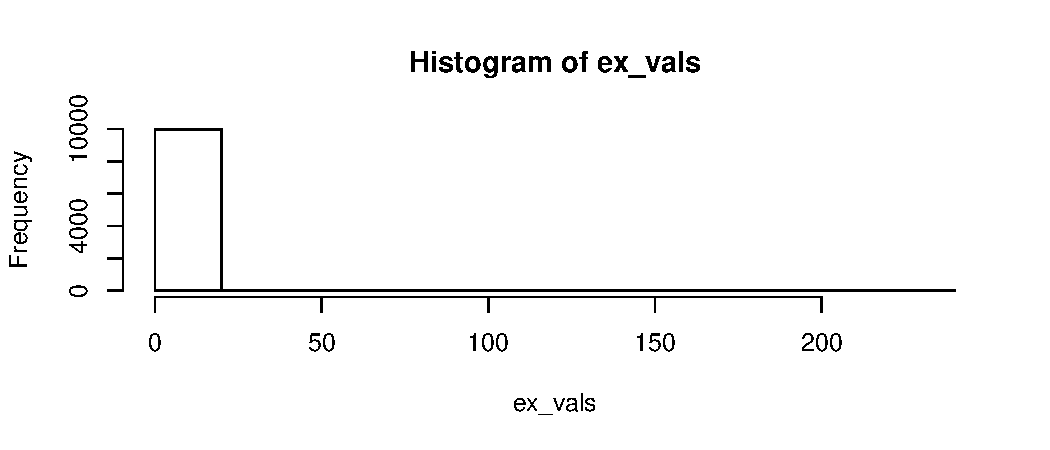
\includegraphics[width=\maxwidth]{figure/unnamed-chunk-3-1} 
\begin{kframe}\begin{alltt}
\hlkwd{hist}\hlstd{(ex_2_vals)}
\end{alltt}
\end{kframe}
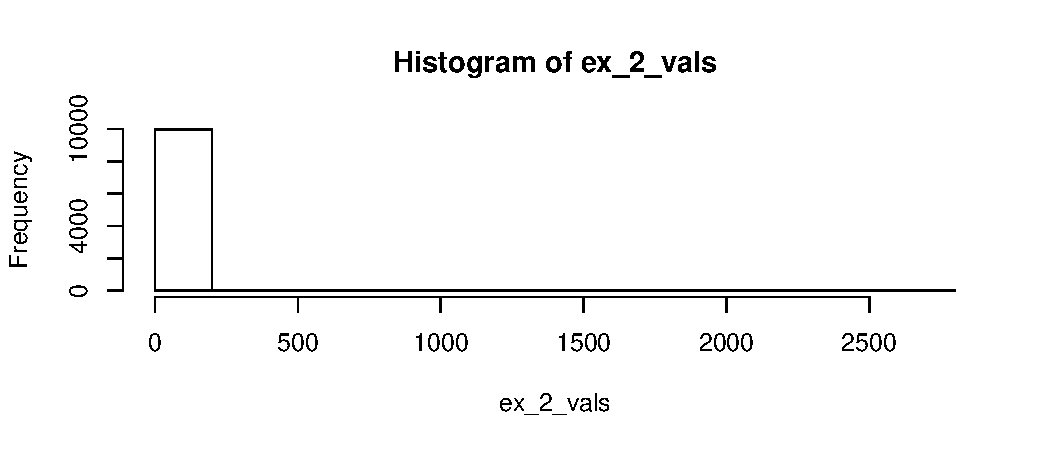
\includegraphics[width=\maxwidth]{figure/unnamed-chunk-3-2} 
\begin{kframe}\begin{alltt}
\hlkwd{hist}\hlstd{(my_weights)}
\end{alltt}
\end{kframe}
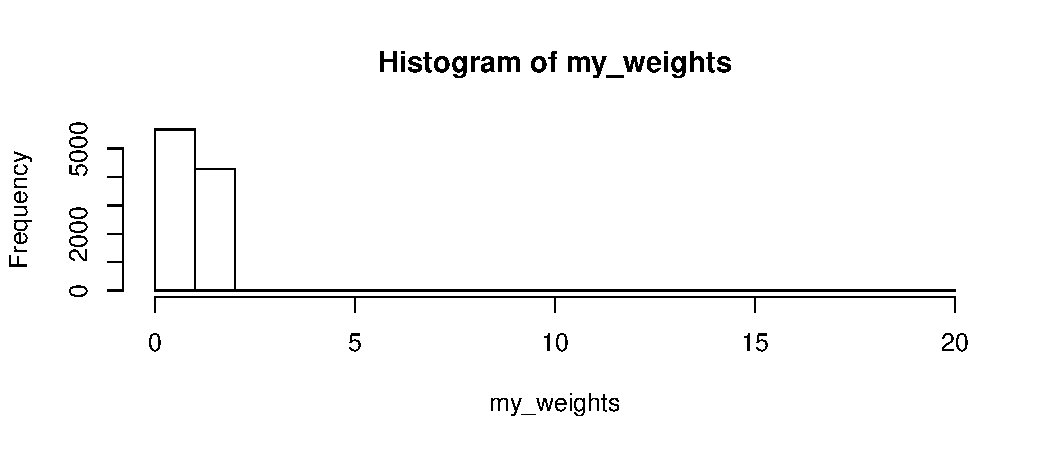
\includegraphics[width=\maxwidth]{figure/unnamed-chunk-3-3} 
\begin{kframe}\begin{alltt}
\hlstd{EX}
\end{alltt}
\begin{verbatim}
## [1] 2.942006
\end{verbatim}
\begin{alltt}
\hlstd{EX2}
\end{alltt}
\begin{verbatim}
## [1] 10.26565
\end{verbatim}
\end{kframe}
\end{knitrout}

The weights here are not as extreme/deviant from the distribution.

\section{}

\subsection{}

Starting for the log likelihood definition given by Harold's section notes:

\begin{align*}
l(\theta, Y) = \frac{n}{2} \log \sigma^2 - \frac{1}{2 \sigma^2} \sum_{i=1}^{c} (Y_{obs,i} - \mu)^2 - c\\
\end{align*}

Take \(Y = Z\), \(\theta = \beta\), and \(\sigma = 1\), from the problem statement.  Then:

\begin{align*}
l(\theta, Y) = -\frac{1}{2} \sum_{i=1}^c (z_i - x_i^T \beta)^2 - c
\end{align*}

So now we can complete:

\begin{align*}
Q(\beta | \beta^{(t)}) &= E[l(\beta, Y) | y_{obs}, \beta^{(t)}]\\
				&= E[\sum_{i=1}^c (z_i - x_i^T \beta)^2 | Y = y_obs, \beta = \beta^{(T)}] + c\\
				&= \frac{1}{2} E[(z - x\beta)^T(z- x\beta)]\\
				&=-\frac{1}{2} \beta^T x^T x \beta + E[\beta^T x^T z] + c'\\
				&= \frac{1}{2}\beta^T x^T x \beta + \beta^T x^T E[z] + c'
\end{align*}

Our observations \(y_i\) will have two values, 0 or 1.  Conditioning on either, our \(z_i\) values will be distributed according to the truncated normal distribution for the mean \(=x_i^T \beta^{(t)}\) and the standard deviation of 1 for ranges from -infinity to 0, and 0 to infinity, respectively.  Then, differential Q, with respect to beta:

\begin{align*}
\frac{\partial Q}{\partial \beta} &= -\beta^T X^T X + (E[x^T z])^T = 0\\
(\beta^T x^T x)^T &= E[x^T z]
\end{align*}
So:

\[ \beta^{(t+1)} = (x^Tx)^{-1} x^T E[z] \]

Where z is advanced from our problem statement for \(y_i\) = 0:

\[ E[z]^{(t+1)} = x_i^T \beta^{(t)} - \frac{\phi(x_i^T \beta^{(t)})}{\Phi(-x_i^T \beta^{(t)})} \]

and for when \(y_i = 1\):

\[ E[z]^{(t+1)} = x_i^T \beta^{(t)} + \frac{\phi(x_i^T \beta^{(t)})}{1 - \Phi(-x_i^T \beta^{(t)})} \]


These form the basis for the implementation of the E/M algorithm that follows.

Citation: Harold's notes, Wikipedia, and lecture notes from STAT 250 at UCLA (Prof. Baines).

\subsection{}

I propose initializing all the \(\beta_i = 0\).  These, signifies a starting probability of 50\% for each occurence.

\subsection{}

\begin{knitrout}
\definecolor{shadecolor}{rgb}{0.969, 0.969, 0.969}\color{fgcolor}\begin{kframe}
\begin{alltt}
\hlcom{# c) the EM algorithm implementation described above, keeping track of iterations}
\hlcom{# for the later part(s) of the question}
\hlstd{Probit_EM} \hlkwb{<-} \hlkwa{function}\hlstd{(}\hlkwc{X}\hlstd{,} \hlkwc{y}\hlstd{,} \hlkwc{beta}\hlstd{,} \hlkwc{epsilon}\hlstd{) \{}
    \hlstd{iter} \hlkwb{<-} \hlnum{0}
    \hlstd{mean} \hlkwb{<-} \hlstd{X} \hlopt \hlstd{beta}
    \hlstd{converge} \hlkwb{<-} \hlnum{FALSE}

    \hlkwa{while} \hlstd{(}\hlopt{!}\hlstd{converge) \{}
        \hlstd{Ez} \hlkwb{<-} \hlstd{mean} \hlopt{-} \hlstd{(}\hlnum{1}\hlopt{-}\hlstd{y)}\hlopt{*}\hlkwd{dnorm}\hlstd{(mean)}\hlopt{/}\hlkwd{pnorm}\hlstd{(}\hlopt{-}\hlstd{mean)} \hlopt{+} \hlstd{y}\hlopt{*}\hlkwd{dnorm}\hlstd{(mean)}\hlopt{/}\hlstd{(}\hlnum{1}\hlopt{-}\hlkwd{pnorm}\hlstd{(}\hlopt{-}\hlstd{mean))}
        \hlstd{former_beta} \hlkwb{<-} \hlstd{beta}
        \hlstd{beta} \hlkwb{<-} \hlkwd{solve}\hlstd{(}\hlkwd{t}\hlstd{(X)} \hlopt \hlstd{X)} \hlopt \hlkwd{t}\hlstd{(X)} \hlopt \hlstd{Ez}
        \hlstd{mean} \hlkwb{<-} \hlstd{X} \hlopt \hlstd{beta}

        \hlstd{iter} \hlkwb{<-} \hlstd{iter} \hlopt{+} \hlnum{1}
        \hlcom{# An arbitrary convergence criterea.}
        \hlkwa{if} \hlstd{(}\hlkwd{max}\hlstd{(}\hlkwd{abs}\hlstd{(beta} \hlopt{-} \hlstd{former_beta))} \hlopt{<} \hlstd{epsilon ) \{}
             \hlstd{converge} \hlkwb{<-} \hlnum{TRUE}
        \hlstd{\}}
    \hlstd{\}}
    \hlkwd{return}\hlstd{(}\hlkwd{c}\hlstd{(beta, iter))}

\hlstd{\}}

\hlcom{# Choose beta as allows us to have the needed SE ratio, and then]}
\hlcom{# build our inputs based on the probit}

\hlstd{beta} \hlkwb{<-} \hlkwd{c}\hlstd{(}\hlnum{3}\hlstd{,}\hlnum{4}\hlstd{,}\hlnum{0}\hlstd{,}\hlnum{0}\hlstd{)}
\hlstd{X} \hlkwb{<-} \hlkwd{cbind}\hlstd{(}\hlnum{1}\hlstd{,} \hlkwd{rnorm}\hlstd{(}\hlkwc{n} \hlstd{=} \hlnum{100}\hlstd{),} \hlkwd{rnorm}\hlstd{(}\hlkwc{n} \hlstd{=} \hlnum{100}\hlstd{),} \hlkwd{rnorm}\hlstd{(}\hlkwc{n} \hlstd{=} \hlnum{100}\hlstd{))}
\hlstd{mean} \hlkwb{<-} \hlstd{X} \hlopt \hlstd{beta}
\hlstd{Z} \hlkwb{<-} \hlkwd{rnorm}\hlstd{(mean,}\hlkwc{sd}\hlstd{=}\hlnum{1}\hlstd{)}
\hlstd{y} \hlkwb{<-} \hlstd{(Z} \hlopt{>} \hlnum{0}\hlstd{)}
\hlstd{iter} \hlkwb{<-} \hlnum{0}

\hlstd{pem} \hlkwb{<-} \hlkwd{Probit_EM}\hlstd{(X, y, beta,} \hlnum{.00001}\hlstd{)}

\hlcom{# Show our resulting betas}

\hlkwd{print}\hlstd{(}\hlstr{"Iterations, and betas, respectively:"}\hlstd{)}
\end{alltt}
\begin{verbatim}
## [1] "Iterations, and betas, respectively:"
\end{verbatim}
\begin{alltt}
\hlkwd{print}\hlstd{(pem[}\hlnum{1}\hlopt{:}\hlnum{4}\hlstd{])}
\end{alltt}
\begin{verbatim}
## [1] -0.24295412  0.02624449  0.14998443  0.09184392
\end{verbatim}
\begin{alltt}
\hlkwd{print}\hlstd{(pem[}\hlnum{5}\hlstd{])}
\end{alltt}
\begin{verbatim}
## [1] 15
\end{verbatim}
\end{kframe}
\end{knitrout}

\subsection{}

Here we write in the log-likelihood directly and maximize.  The EM converges faster.  The details for the standard error are shown below.

\begin{knitrout}
\definecolor{shadecolor}{rgb}{0.969, 0.969, 0.969}\color{fgcolor}\begin{kframe}
\begin{alltt}
\hlcom{# d) how to check answer by maximizing the log-likelihood}
\hlcom{# Defining our log-likelihood for the probit}

\hlstd{llp} \hlkwb{<-} \hlkwa{function}\hlstd{(}\hlkwc{beta}\hlstd{,} \hlkwc{x}\hlstd{,} \hlkwc{y}\hlstd{) \{}
  \hlstd{mean} \hlkwb{<-} \hlstd{x} \hlopt \hlstd{beta}
  \hlstd{loglike} \hlkwb{<-} \hlkwd{sum}\hlstd{(y} \hlopt{*} \hlkwd{log}\hlstd{(}\hlkwd{pnorm}\hlstd{(mean))} \hlopt{+} \hlstd{(}\hlnum{1}\hlopt{-}\hlstd{y)} \hlopt{*} \hlkwd{log}\hlstd{(}\hlkwd{pnorm}\hlstd{(}\hlopt{-}\hlstd{mean)))}
  \hlkwd{return}\hlstd{(loglike)}
\hlstd{\}}

\hlcom{# Perform the optimization (fnscale = -1 gives the maximum), using BFGS}

\hlstd{llp_optim} \hlkwb{=} \hlkwd{optim}\hlstd{(beta, llp,} \hlkwc{x}\hlstd{=X,} \hlkwc{y}\hlstd{=y,} \hlkwc{control}\hlstd{=}\hlkwd{list}\hlstd{(}\hlkwc{fnscale}\hlstd{=}\hlopt{-}\hlnum{1}\hlstd{,} \hlkwc{maxit}\hlstd{=}\hlnum{1000}\hlstd{,} \hlkwc{reltol}\hlstd{=}\hlnum{.00001}\hlstd{),} \hlkwc{method}\hlstd{=}\hlstr{"BFGS"}\hlstd{)}
\hlstd{llp_optim}\hlopt{$}\hlstd{par}
\end{alltt}
\begin{verbatim}
## [1] -0.24304582  0.02624396  0.14988449  0.09178409
\end{verbatim}
\begin{alltt}
\hlstd{llp_optim}\hlopt{$}\hlstd{counts}
\end{alltt}
\begin{verbatim}
## function gradient 
##       38        9
\end{verbatim}
\begin{alltt}
\hlcom{# A brief illustration showing how we found the beta1 / se(beta1) --}
\hlcom{# Also confirming both EM and LL solutions are correct with the GLM, and showing}
\hlcom{# that we have the correct se ratio.}

\hlstd{glm_probit} \hlkwb{<-} \hlkwd{glm}\hlstd{(y} \hlopt{~} \hlstd{X[,}\hlnum{2}\hlstd{]} \hlopt{+} \hlstd{X[,}\hlnum{3}\hlstd{]} \hlopt{+} \hlstd{X[,}\hlnum{4}\hlstd{],} \hlkwc{family} \hlstd{=} \hlkwd{binomial}\hlstd{(}\hlkwc{link} \hlstd{=} \hlstr{"probit"}\hlstd{))}
\hlstd{glm_probit}\hlopt{$}\hlstd{coefficients}
\end{alltt}
\begin{verbatim}
## (Intercept)      X[, 2]      X[, 3]      X[, 4] 
## -0.24295458  0.02623951  0.14998252  0.09184285
\end{verbatim}
\begin{alltt}
\hlkwd{summary}\hlstd{(glm_probit)}
\end{alltt}
\begin{verbatim}
## 
## Call:
## glm(formula = y ~ X[, 2] + X[, 3] + X[, 4], family = binomial(link = "probit"))
## 
## Deviance Residuals: 
##     Min       1Q   Median       3Q      Max  
## -1.3009  -1.0057  -0.8737   1.2723   1.5879  
## 
## Coefficients:
##             Estimate Std. Error z value Pr(>|z|)  
## (Intercept) -0.24295    0.13334  -1.822   0.0685 .
## X[, 2]       0.02624    0.12290   0.213   0.8309  
## X[, 3]       0.14998    0.12573   1.193   0.2329  
## X[, 4]       0.09184    0.13011   0.706   0.4803  
## ---
## Signif. codes:  0 '***' 0.001 '**' 0.01 '*' 0.05 '.' 0.1 ' ' 1
## 
## (Dispersion parameter for binomial family taken to be 1)
## 
##     Null deviance: 133.75  on 99  degrees of freedom
## Residual deviance: 131.69  on 96  degrees of freedom
## AIC: 139.69
## 
## Number of Fisher Scoring iterations: 4
\end{verbatim}
\end{kframe}
\end{knitrout}

\section{}

We print a few graphs for the last coordinate value fixed at -1, -2, and -3 (the negative values seemed to give rise to the helical shape I believe was intended).  NLM and OPTIM give results in common, but vary both in terms of total number of minimia given as well as minima chosen.  The global minimum seems to be at (1, 0, 0).

\begin{knitrout}
\definecolor{shadecolor}{rgb}{0.969, 0.969, 0.969}\color{fgcolor}\begin{kframe}
\begin{alltt}
\hlkwd{attach}\hlstd{(mtcars)}
\end{alltt}


{\ttfamily\noindent\itshape\color{messagecolor}{\#\# The following objects are masked from mtcars (pos = 3):\\\#\# \\\#\#\ \ \ \  am, carb, cyl, disp, drat, gear, hp, mpg, qsec, vs, wt}}\begin{alltt}
\hlkwd{par}\hlstd{(}\hlkwc{mfrow}\hlstd{=}\hlkwd{c}\hlstd{(}\hlnum{3}\hlstd{,}\hlnum{3}\hlstd{))}

\hlcom{# Code copy + pasted from Chris' problme statement}

\hlstd{theta} \hlkwb{<-} \hlkwa{function}\hlstd{(}\hlkwc{x1}\hlstd{,}\hlkwc{x2}\hlstd{)} \hlkwd{atan2}\hlstd{(x2, x1)}\hlopt{/}\hlstd{(}\hlnum{2}\hlopt{*}\hlstd{pi)}

\hlstd{f} \hlkwb{<-} \hlkwa{function}\hlstd{(}\hlkwc{x}\hlstd{) \{}
  \hlstd{f1} \hlkwb{<-} \hlnum{10}\hlopt{*}\hlstd{(x[}\hlnum{3}\hlstd{]} \hlopt{-} \hlnum{10}\hlopt{*}\hlkwd{theta}\hlstd{(x[}\hlnum{1}\hlstd{],x[}\hlnum{2}\hlstd{]))}
  \hlstd{f2} \hlkwb{<-} \hlnum{10}\hlopt{*}\hlstd{(}\hlkwd{sqrt}\hlstd{(x[}\hlnum{1}\hlstd{]}\hlopt{^}\hlnum{2}\hlopt{+}\hlstd{x[}\hlnum{2}\hlstd{]}\hlopt{^}\hlnum{2}\hlstd{)}\hlopt{-}\hlnum{1}\hlstd{)}
  \hlstd{f3} \hlkwb{<-} \hlstd{x[}\hlnum{3}\hlstd{]}
  \hlkwd{return}\hlstd{(f1}\hlopt{^}\hlnum{2}\hlopt{+}\hlstd{f2}\hlopt{^}\hlnum{2}\hlopt{+}\hlstd{f3}\hlopt{^}\hlnum{2}\hlstd{)}
\hlstd{\}}

\hlcom{# Show three graphs for three different z conditions}

\hlkwd{print}\hlstd{(}\hlstr{"For a constant z of -1, -2, and -3..."}\hlstd{)}
\end{alltt}
\begin{verbatim}
## [1] "For a constant z of -1, -2, and -3..."
\end{verbatim}
\begin{alltt}
\hlkwa{for} \hlstd{(q} \hlkwa{in} \hlnum{1}\hlopt{:}\hlnum{3}\hlstd{) \{}
    \hlstd{x}\hlkwb{=}\hlkwd{seq}\hlstd{(}\hlopt{-}\hlnum{10}\hlstd{,}\hlnum{10}\hlstd{,}\hlnum{1}\hlstd{)}
    \hlstd{y}\hlkwb{=}\hlkwd{seq}\hlstd{(}\hlopt{-}\hlnum{10}\hlstd{,}\hlnum{10}\hlstd{,}\hlnum{1}\hlstd{)}
    \hlstd{x_len}\hlkwb{=} \hlkwd{length}\hlstd{(x)}
    \hlstd{y_len} \hlkwb{=} \hlkwd{length}\hlstd{(y)}
    \hlstd{z}\hlkwb{=}\hlkwd{array}\hlstd{(}\hlnum{0}\hlstd{,}\hlkwc{dim}\hlstd{=}\hlkwd{c}\hlstd{(x_len,y_len))}

    \hlkwa{for} \hlstd{(i} \hlkwa{in} \hlnum{1}\hlopt{:}\hlstd{x_len)} \hlkwa{for} \hlstd{(j} \hlkwa{in} \hlnum{1}\hlopt{:}\hlstd{y_len) z[i,j]} \hlkwb{=} \hlkwd{f}\hlstd{(}\hlkwd{c}\hlstd{(x[i],y[j],}\hlopt{-}\hlstd{q))}

    \hlkwd{persp}\hlstd{(x, y, z,} \hlkwc{phi} \hlstd{=} \hlnum{20}\hlstd{,} \hlkwc{theta} \hlstd{=} \hlnum{40}\hlstd{)}
    \hlkwd{contour}\hlstd{(x, y, z)}
    \hlkwd{image}\hlstd{(x, y, z)}
\hlstd{\}}
\end{alltt}
\end{kframe}
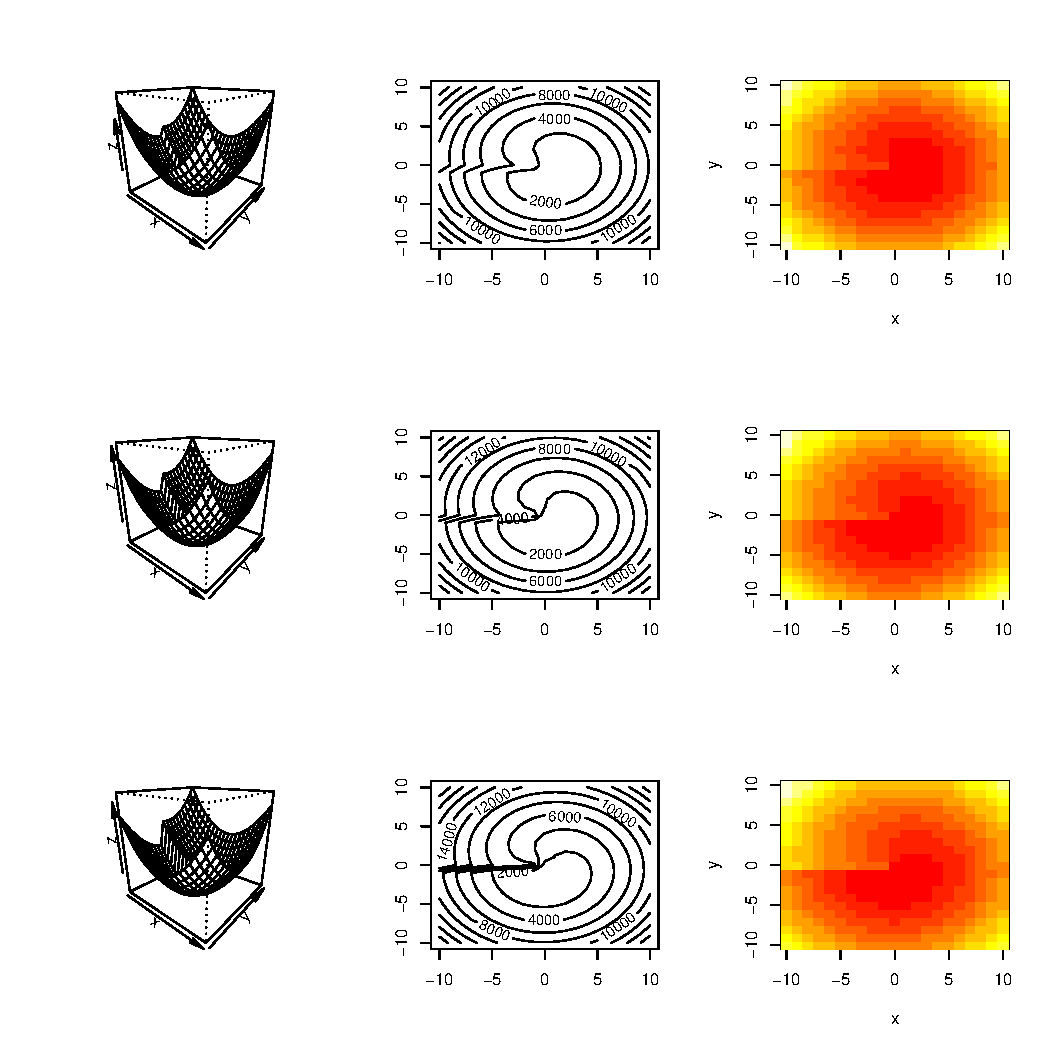
\includegraphics[width=\maxwidth]{figure/unnamed-chunk-6-1} 
\begin{kframe}\begin{alltt}
\hlcom{# Comparing optimization methods for all possible values of (x, y, z) for all integers between -10 and 10 (moving by 2).}

\hlstd{x_range} \hlkwb{=} \hlkwd{seq}\hlstd{(}\hlopt{-}\hlnum{10}\hlstd{,}\hlnum{10}\hlstd{,}\hlnum{2}\hlstd{)}
\hlstd{y_range} \hlkwb{=} \hlkwd{seq}\hlstd{(}\hlopt{-}\hlnum{10}\hlstd{,}\hlnum{10}\hlstd{,}\hlnum{2}\hlstd{)}
\hlstd{z_range} \hlkwb{=} \hlkwd{seq}\hlstd{(}\hlopt{-}\hlnum{10}\hlstd{,}\hlnum{10}\hlstd{,}\hlnum{2}\hlstd{)}

\hlcom{# Initialize empty results for later}
\hlstd{optim_results} \hlkwb{=} \hlkwd{c}\hlstd{()}
\hlstd{nlm_results} \hlkwb{=} \hlkwd{c}\hlstd{()}

\hlkwa{for} \hlstd{(xi} \hlkwa{in} \hlstd{x_range) \{}
  \hlkwa{for} \hlstd{(yi} \hlkwa{in} \hlstd{y_range) \{}
    \hlkwa{for} \hlstd{(zi} \hlkwa{in} \hlstd{z_range) \{}
      \hlstd{out.optim} \hlkwb{<-} \hlkwd{optim}\hlstd{(}\hlkwd{c}\hlstd{(xi,yi,zi),} \hlkwc{fn} \hlstd{= f)}
      \hlstd{out.nlm} \hlkwb{<-} \hlkwd{nlm}\hlstd{(}\hlkwc{p}\hlstd{=}\hlkwd{c}\hlstd{(xi,yi,zi),} \hlkwc{f} \hlstd{= f)}
      \hlcom{# We need to round agressively to get unique results}
      \hlstd{optim_results} \hlkwb{<-} \hlkwd{rbind}\hlstd{(optim_results,} \hlkwd{round}\hlstd{(}\hlkwd{c}\hlstd{(out.optim}\hlopt{$}\hlstd{par, out.optim}\hlopt{$}\hlstd{value),}\hlnum{2}\hlstd{))}
      \hlstd{nlm_results} \hlkwb{<-} \hlkwd{rbind}\hlstd{(nlm_results,} \hlkwd{round}\hlstd{(}\hlkwd{c}\hlstd{(out.nlm}\hlopt{$}\hlstd{estimate, out.nlm}\hlopt{$}\hlstd{minimum),}\hlkwc{digits}\hlstd{=}\hlnum{2}\hlstd{))}
    \hlstd{\}}
  \hlstd{\}}
\hlstd{\}}

\hlcom{# Just give the unique results}

\hlkwd{print}\hlstd{(}\hlkwd{unique}\hlstd{(optim_results))}
\end{alltt}
\begin{verbatim}
##        [,1]  [,2]  [,3]    [,4]
##  [1,]  1.00  0.00  0.00    0.00
##  [2,]  1.00 -0.01 -0.01    0.00
##  [3,]  1.00  0.01  0.01    0.00
##  [4,]  1.00  0.00  0.01    0.00
##  [5,] -1.00 -0.03 -4.90   24.27
##  [6,]  1.00 -0.01 -0.02    0.00
##  [7,]  1.00  0.00 -0.01    0.00
##  [8,]  0.96  0.42  0.64    0.64
##  [9,] -6.33  0.00  2.00 3748.44
## [10,]  1.00  0.01  0.02    0.00
## [11,]  0.94 -0.44 -0.71    0.72
## [12,] -0.50  0.00 -7.19  557.96
## [13,]  1.00 -0.02 -0.03    0.00
## [14,] -1.00  0.00 -4.95   24.74
## [15,]  1.01 -0.05 -0.08    0.01
## [16,] -1.51  0.00 -5.38   69.05
## [17,] -4.80  0.00  0.93 3098.65
## [18,] -0.48  0.88  3.28   10.76
## [19,]  1.00  0.05  0.08    0.01
## [20,]  1.00  0.02  0.03    0.00
## [21,] -1.00  0.00  4.95   24.72
## [22,]  1.01  0.01  0.01    0.01
## [23,]  0.00  0.00  6.98  539.05
## [24,]  0.96  0.28  0.46    0.21
## [25,] -0.64  0.00 -5.43   60.81
## [26,]  0.97  0.26  0.41    0.17
## [27,] -2.38  0.00  3.47  437.03
## [28,]  1.00 -0.02 -0.04    0.00
## [29,] -1.23  0.00 -5.18   35.51
## [30,]  1.00 -0.06 -0.09    0.01
## [31,]  1.00 -0.07 -0.11    0.01
## [32,]  1.00  0.03  0.05    0.00
## [33,] -1.18  0.00 -5.11   30.65
## [34,]  0.99  0.04  0.06    0.01
## [35,]  1.00  0.02  0.04    0.00
## [36,]  1.00  0.06  0.09    0.01
## [37,]  1.00  0.04  0.06    0.00
## [38,]  1.00  0.06  0.10    0.01
## [39,]  1.00  0.03  0.06    0.00
## [40,] -1.00  0.00 -4.95   24.73
## [41,]  1.00 -0.03 -0.05    0.00
## [42,]  1.00 -0.04 -0.07    0.01
## [43,]  1.00 -0.06 -0.10    0.01
## [44,]  0.98 -0.19 -0.30    0.09
## [45,] -0.60  0.00  6.06  165.01
## [46,]  1.00  0.03  0.04    0.00
## [47,]  0.00  0.00  7.00  549.76
\end{verbatim}
\begin{alltt}
\hlkwd{print}\hlstd{(}\hlkwd{unique}\hlstd{(nlm_results))}
\end{alltt}
\begin{verbatim}
##        [,1]  [,2]   [,3]    [,4]
##  [1,]  1.00  0.00   0.00    0.00
##  [2,] -4.00  0.00   6.00 1036.00
##  [3,] -0.75  0.00   5.05   32.09
##  [4,] -1.37  0.00  -6.25  210.10
##  [5,] -2.00  0.00   6.00  236.00
##  [6,] -2.00  0.00   8.00 1064.00
##  [7,] -2.00  0.00  10.00 2700.00
##  [8,] -1.37  0.00   6.25  210.10
##  [9,] -1.08  0.00  -5.03   25.98
## [10,]  0.00  0.00 -10.00 5824.02
## [11,]  0.00 -0.01  -8.00 3187.65
## [12,]  0.00  0.00  -6.00 1359.99
## [13,]  0.00  0.00  -4.00  340.35
## [14,]  0.00  0.00  -2.00  128.68
## [15,]  0.00  0.00   0.00  100.00
## [16,]  0.00  0.01   2.00  127.34
## [17,]  0.00  0.01   4.00  339.54
## [18,]  0.00  0.00   6.00 1359.95
## [19,]  0.00  0.01   8.00 3187.61
## [20,]  0.00  0.01  10.00 5823.28
## [21,] -0.39  0.00   5.47   89.26
## [22,] -1.00  0.00  -4.95   24.75
## [23,] -0.63  0.00   5.42   60.61
## [24,] -0.55  0.00   5.49   74.56
## [25,] -0.55  0.00  -5.49   74.56
\end{verbatim}
\end{kframe}
\end{knitrout}



\end{document}
